\section{Theorie}
Um Informationen mit Hilfe von elektromagnetischen Wellen übertragen zu können, werden Verfahren benötigt um diesen Wellen Informationen aufprägen zu können. Solche Verfahren werden Modulationsverfahren genannt; das Rückgewinnen der Informationen aus der modulierten Welle nennt man Demodulation.

Die Hochfrequenztechnik kennt eine Reihe von Modulationsverfahren, welche unter Ausnutzung einer periodischen Änderung von Amplitude, Frequenz oder Phase einer Trägerwelle dieser Informationen aufprägen.

\subsection{Amplitudenmodulation}
Die einfachste Form der Amplitudenmodulation lässt die Amplitude einer hochfrequenten Trägerwelle $U_T(t)$ im Rythmus einer niederfrequenten Modulationswelle $U_M(t)$ variieren. Die Trägerwelle besitzt die Frequenz $\omega_T$ und die Modulationswelle die
Frequenz $\omega_M$.

Die amplitudenmodulierte Schwingung soll dann eine mit $\omega_M$ varrierende Amplitude

\begin{equation}
U_{3}(t) = U_T (1 + m \cos( \omega_M t))\cos(\omega_T t)
\label{eq:AmMod}
\end{equation} 

besitzen, wobei $m = \gamma U_M$ den  Modulationsgrad der Schwingung beschreibt.

\begin{figure}
	\centering
	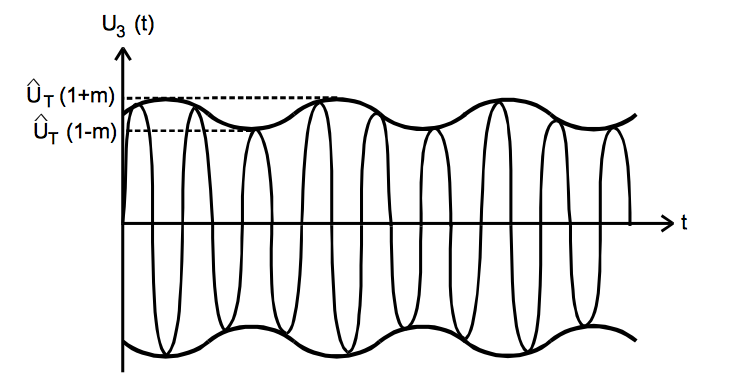
\includegraphics[width=\textwidth]{img/Abb1.png}
	\caption{Zeitabhängigkeit der Signalspannung eines Amplitudenmodulierten Signals \cite{FP}}
\end{figure}

Wird durch geeignete Umformung oder Fouriertransformation das Frequenzspektrum der Schwinung analysiert, fällt auf, dass in diesem einfachen Fall bereits drei Frequenzen beteiligt sind:

\begin{equation}
U_{3}(t) = U_T ( \cos(\omega_T t) + \frac{1}{2}m\cos(\omega_T + \omega_M)t + \frac{1}{2}m\cos(\omega_T - \omega_M)t).
\label{eq:FreqAmMod}
\end{equation}

\begin{figure}
	\centering
	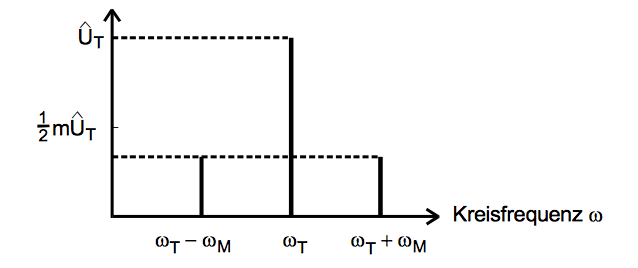
\includegraphics[width=\textwidth]{img/Abb2.png}
	\caption{Frequenzspektrum einer Amplitudenmodulierten Schwingung \cite{FP}}
\end{figure}

Die Frequenz bei $\omega_T$ nennt man Trägerfrequenz, diese trägt keine Information und stellt einen dissipativen Anteil dar, welcher in der Praxis unerwünscht ist. Auch beschreiben die beiden Seitenbänder bei $\omega_T - \omega_M$ und $\omega_T + \omega_M$die gleichen Informationen. Somit ist es üblich, eines der beiden Seitenbänder durch geeignete Filter zu unterdrücken.
Wird die Trägerfrequenz und ein Seitenband unterdrückt, wird auch von Einseitenbandmodulation mit Trägerunterdrückung gesprochen.
Die großen Nachteile der Amplitudenmodulation bestehen in ihrer geringen Störsicherheit und geringen Verzerrungsfreiheit.

\subsection{Frequenzmodulation}
Anders als bei der Amplitudenmodulation wird bei der Frequenzmodulation die momentane Schwingungsfrequenz im Rythmus des Modulationssignales variiert.

\begin{equation}
U(t)= U\sin(\omega_T t + m \frac{\omega_T}{\omega_M} \cos(\omega_M t))
\label{eq:FreqMod}
\end{equation}

Durch Differentiation des Arguments des Sinuses ergibt sich die Momentanfrequenz

\begin{equation}
f(t) = \frac{\omega_T}{2\pi}(1-m\sin(\omega_M t))
\label{eq:momFreq}
\end{equation}

der Schwingung, wobei $m$ wieder den Modulationsgrad und $\frac{m\omega_T}{2\pi}$ den Frequenzhub geschreibt. Der Frequenzhub ist es Maß dafür, wie Stark die Schwinungsfrequenz varriert. Im folgenden ist eine Schmalband-Frequenzmoduation zu sehen, welche sich durch

\begin{equation}
m\frac{\omega_T}{\omega_M} << 1
\end{equation}

auszeichnet.

\begin{figure}
	\centering
	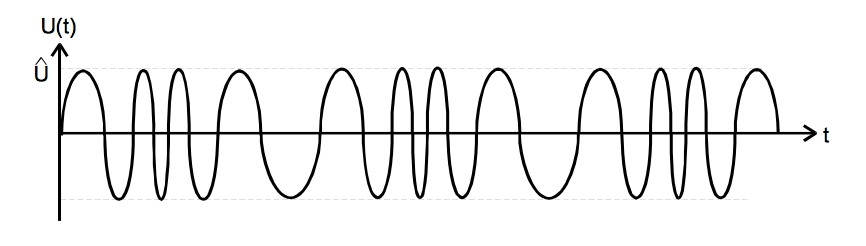
\includegraphics[width=\textwidth]{img/Abb3.png}
	\caption{Zeitlicher Verlauf einer frequenzmodulierten Schwingung \cite{FP}}
\end{figure}

Durch geeignete Umformung oder Fouriertransfromation ist ersichtlich, dass auch das Frequenzspektrum der Frequenzmodulation sich aus drei Frequenzen zusammensetzt.

\begin{equation}
U(t) = U(\sin(\omega_T t) + \frac{m\omega_T}{2\omega_M}\cos(\omega_T + \omega_M) t \frac{m\omega_T}{2\omega_M}\cos(\omega_T - \omega_M) t)
\label{eq:FreqFreqMod}
\end{equation}

Es fällt auf, dass die beiden Seitenbänder im Fall der Frequenzmodulation um $\frac{\pi}{2}$ gegebüber der Trägerschwingung vershoben sind. Es ist anzumerken, dass das o.g. Frequenzspektrum nur im Fall der schwach frequenzmodulierten Schwingung

\begin{equation}
\frac{m\omega_T}{\omega_M} << 1
\end{equation}

Gültigkeit besitzt. Im Fall der starken Frequenzmodulation

\begin{equation}
m\omega_T \approx \omega_M
\end{equation}

besitzt das Frequenzspektrum eine komplexere Darstellung der Form

\begin{equation}
U(t) = U \sum_{n=-\inf}^{+\inf} J_{n}(\frac{m\omega_T}{\omega_M})\sin(\omega_T + n\omega_M)t,
\end{equation}

wobei $J_n$ die Besselsche Funktion n-ter Ordnung ist. Es zeigt sich, dass für hohe Modulationsgrade das Frequenzspektrum im Prinzip bis zu beliebig hohen Frequenzen reicht. Es reicht jedoch in der Praxis nur Frequenzen in der Nähe der Trägerfrequenz zu berücksichtigen, da

\begin{equation}
J_{\pm n}(x) \approx \frac{1}{\sqrt{2\pi n}}(\frac{ex}{2n})^n
\end{equation}

mit wachsender Ordnungszahl $n$ und $x \leq 1$ schnell gegen null geht.

\subsection{Modulationsschaltungen}
Um die Amplitude einer Trägerschwingung wie in \autoref{eq:AmMod} zu modulieren, wird ein Bauteil benötigt, welches das Produkt aus zwei Eingangspannungen bilden kann. Grundsätzlich ist das mit jedem Bauteil möglich, welches eine nichtlineare Kennlinie besitzt.
Eine solche Schaltung kann z.B. mit Hilfe einer Diode gemäß \autoref{abb:simpleMod} realisiert werden.

\begin{figure}
	\centering
	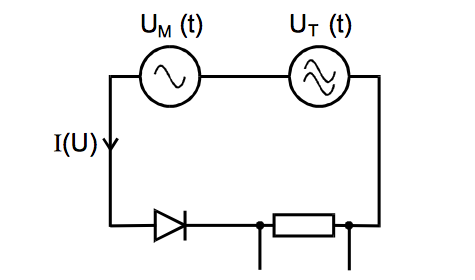
\includegraphics[width=\textwidth]{img/Abb4.png}
	\caption{Primitive Modulatorschaltung \cite{FP}}
	\label{abb:simpleMod}
\end{figure}

Wird die Summe von Träger- und Modulatorspannung für die Spannung in die Potzenreihenentwicklung der Diodenkennlinie eingesetzt

\begin{equation}
I(U_T + U_M) = a_0 + a_1(U_T + U_M) + a_2(U_T^2 + U_M^2) + 2a_2 U_T U_M + ...
\end{equation}

liefert das vierte Reihenglied das geforderte Produkt. Es fällt auf, dass zusätzliche Störterme aufreten, deren Frequenzen  $\omega_M, 2\omega_M und 2\omega_T$ allerdings weit außerhalb des zu übertragenden Frequenzbandes $\omega_T - \omega_M$ bis $\omega_T + \omega_M$ liegen, sodass diese mit einem geeigneten Bandfilter unterdückt werden können.
Durch das Erzeugen der vielen nicht genutzten Frequenzen ist so eine Schaltung sehr unökonomisch. Es ist wünschenswert das die störenden Frequenzanteile erst gar nicht erzeugt werden.

\subsubsection{Der Ringmodulator}
Der Ringmodulator besteht, wie der Name bereits andeutet, aus einem Ring von vier zusammengeschaltet Dioden.

\begin{figure}
	\centering
	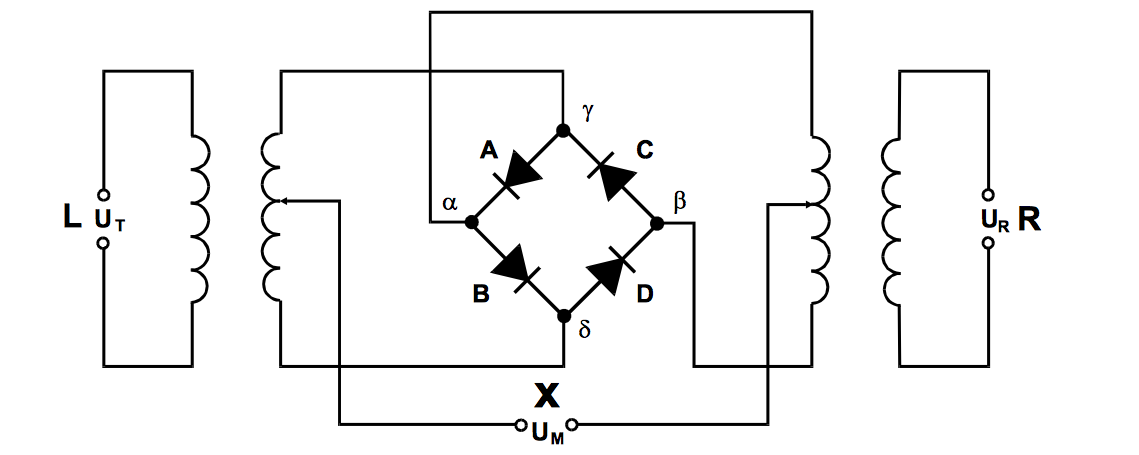
\includegraphics[width=\textwidth]{img/Abb5.png}
	\caption{Schaltung eines Ringmodulators \cite{FP}}
	\label{abb:ringMod}
\end{figure}

Diese Schaltung ist in der Lage, das Produkt von Träger und Modulationssignal zu bilden ohne störende parasitäre Frequenzanteile zu erzeugen. Die abgenommene Spannung ist direkt proportional zum Produkt der Eingangsspannungen.

\begin{equation}
U_R(t) = \gamma U_M(t) \cdot U_T(t)
\label{eq:ringMod}
\end{equation}

Es ist anzumerken, dass $\gamma$ die Einehit $\frac{1}{\text{V}}$ besitzt. Es ist direkt ersichtich, dass der Ringmodulator die Trägerabstrahlung unterdrückt. Werden zwei Cosinus-Signale für $U_T$ und $U_M$ mit den Frequenzen $\omega_T$ und $\omega_M$ in \ref{eq:ringMod} eingesetzt, folgt

\begin{equation}
U_R(t) = \gamma U_T U_M \frac{1}{2}\cos((\omega_T + \omega_M)t + \phi) + \gamma U_T U_M \frac{1}{2} \cos((\omega_T - \omega_M)t - \phi).
\end{equation}

Wie bereits angesprochen fehlt in diesem Frequenzspektrum der Trägeranteil $\omega_T$.

\subsubsection{Frequenzmodulator mit geringem Frequenzhub}
Um einen Frequenzmodulator mit geringem Frequenzhub zu realisieren wird ein Ringmodulator genutzt, jedoch wird, wie aus \autoref{eq:FreqFreqMod} ersichtlich ist, ein $\frac{\pi}{2}$ Phasenschieber notwendig. Dieser wird mit Hilfe eines Iso-T Leistungsteiler parallel neben dem Ringmodulator angeordnet. Die Schaltung ist in \autoref{gering_f-hub} abgebildet.

\begin{figure}
	\centering
	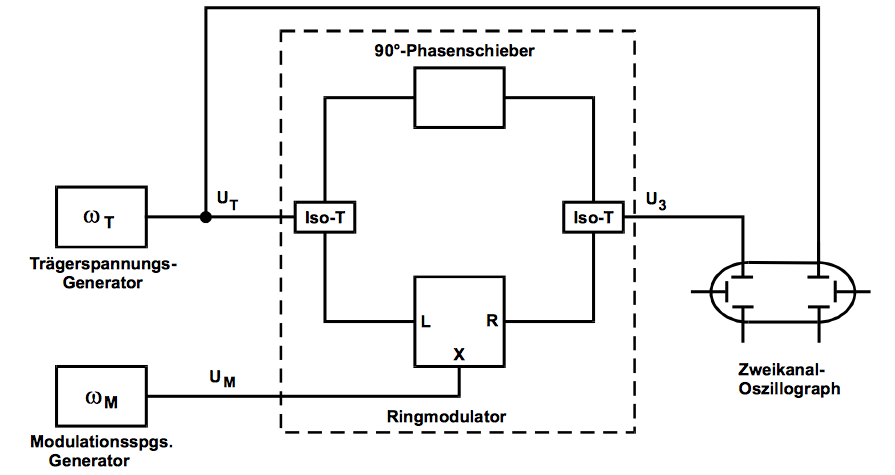
\includegraphics[width=\textwidth]{img/Abb7.png}
	\caption{Frequenzmodulator mit geringem Frequenzhub \cite{FP}}
	\label{gering_f-hub}
\end{figure}

Der Phasenschieber wird mit Hilfe eines Laufzeitkabels realsiert.

\subsection{Demodulationsschaltungen}
\subsubsection{Demodulation amplitudenmodulierter Schwingungen}
Mit Demodulatorschaltungen ist es möglich aus einem modulierten Signal die Modulationsfrequenz $\omega_M$ zurück zu gewinnen.
Wird am einen Eingang eines Ringmodulators ein Signal mit den Frequenzen $\omega_T - \omega_M$ und $\omega_T + \omega_M$ angelegt und am anderen Eingang das Trägersignal mit $\omega_T$, so liefert der Ausgang der Schaltung ein Signal mit
$\omega_M$, $2\omega_T - \omega_M$ und $2\omega_T + \omega_M$. Alle von der Modulationsfrequenz abweichenden Signalanteile lassen sich mit Hilfe eines geeigneten Bandpasses gut unterdrücken, so dass am Ausgang nur noch ein Signal mit der Modulationsfrequenz $\omega_M$ anliegt. Ein Problem welches sich bei der Demodulation stellt ist, dass ein Trägersignal benötigt wird, welches phasenstarr mit dem Trägersignal des Senders gekoppelt sein muss. Um eine solche Kopplung zu gewährleisten wird i.A. ein Phasenregelkreis oder PLL-Schaltung verwendet. 

\begin{figure}
	\centering
	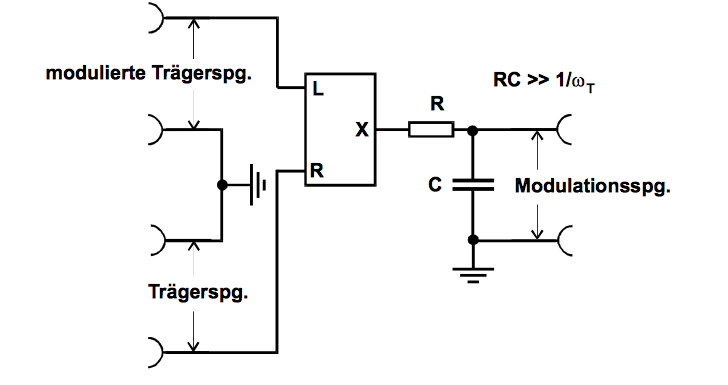
\includegraphics[width=\textwidth]{img/Abb8.png}
	\caption{Demodulation mit Gleichrichter und Iso-T \cite{FP}}
	\label{iso-t}
\end{figure}

Es ist möglich die Problematik der festen Phasenbeziehung zwischen der Signal und Referenzspannung mit Hilfe einer Gleichrichter-Diode 
zu vermeiden.

\begin{figure}
	\centering
	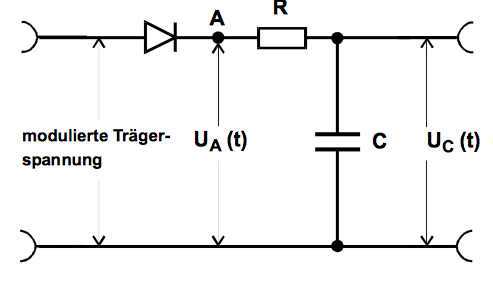
\includegraphics[width=\textwidth]{img/Abb9.png}
	\caption{Demodulation mit Gleichrichter-Diode \cite{FP}}
	\label{fig:9}
\end{figure}

Die Gleichrichter-Diode in \autoref{gleichrichter} schneidet sämtliche negative Halbwellen ab, sodass nach der Diode eine gleichgerichtete, modulierte Hochfrequenz-Spannung abgegeriffen werden kann. Die enthaltenen hochfrequenten Anteile mit den Frequenzen $\omega_T$, $2\omega_T$,
$4\omega_T$ u.v.m. lassen sich mit einem Tiefpass unterdrücken, so dass am Ausgang die Modulationsspannung abgegriffen werden kann.

\begin{figure}
	\centering
	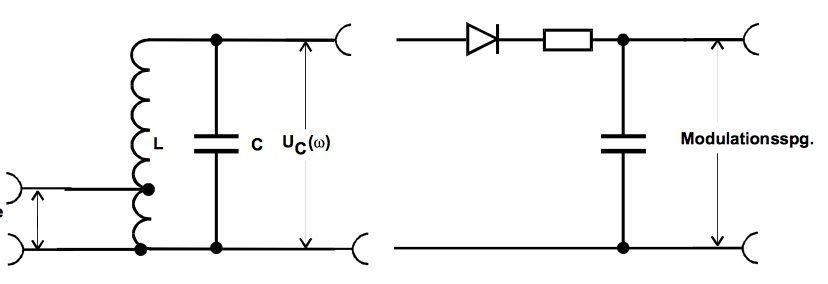
\includegraphics[width=\textwidth]{img/Abb12.png}
	\caption{Negative Halbwellen werden mit der Diode abgeschnitten, der Tiefpass entfernt hochfrequente Anteile. \cite{FP}}
	\label{gleichrichter}
\end{figure}

Problematisch ist jedoch, dass die Diode eine exponentielle Kennline besitzt. Die Abweichung vom gewünschten linearen Verhalten begründet Verzerrungen in der Rückgewinnung des Modulationssignales. Dieses Problemm lässt sich in den Griff bekommen, indem mit geringen Modulationsgraden, also kleinen Auslenkungen gearbeitet wird oder eine Gegentaktschaltung verwendet wird.

\subsubsection{Demodulation frequenzmodulierter Schwingungen}
Um das Modulationssignal aus einer frequenzmodulierten Schwingung gewinnen zu können bietet sich ein so.g Flankenmodulator an.

\begin{figure}
	\centering
	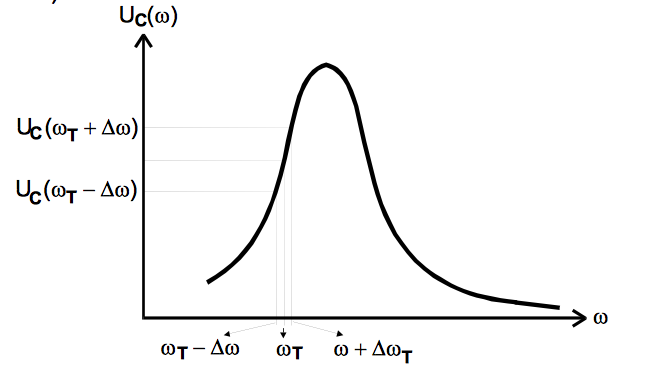
\includegraphics[width=\textwidth]{img/Abb13.png}
	\caption{Die Resonanzfrequenz des Schwingkreises wird so eingestellt, dass die Trägerfrequenz auf der steilen Flanke der Resonanzkurve liegt. \cite{FP}}
	\label{resonanzkurve}
\end{figure}

Der Flankenmodulator besteht im wesentlichen aus einem Schwingkreis, in welchem die Frequenzabhängigkeit der Kondensatorspannung im Falle erzungener Schwingung ausgenutzt wird. Hierfür wird die Resonanzfrequenz des Schwingkreises so eingestellt, dass die Trägerfrequenz $\omega_T$ mitten in der steilen Flanke der Resonanzkurve liegt (\autoref{resonanzkurve}). Ändert sich nun in Folge der Frequenzmodulation die Momentanfrequenz der modulierten Schwingung, so entsteht am Ausgang des Schwingkreises eine hochfrequente Spannung, deren Amplitude im Rhytmus der Modulation schwangt. Somit wurde die Frequenzmodulation in eine Amplitudenmodulation überführt, welche bereites behandelt wurde.